\documentclass{mwart} 
\usepackage[polish]{babel} 
\usepackage[utf8]{inputenc} 
\usepackage{polski} 
\usepackage[T1]{fontenc} 
\usepackage{graphicx}

\usepackage[margin=1cm]{geometry}




\frenchspacing 

\usepackage{indentfirst} 
\title{\Huge{Sprawozdanie z laboratorium nr 4 \\
ALGORYTMY SORTUJĄCE}}
\author{Agnieszka Wiśniewska, nr albumu: 200466}
\date{23.03.2014} 
\begin{document}

\maketitle

\section{Opis zadania\label{wstep}}

Zadaniem do wykonania było przygotowanie programu mierzącego czas wykonywania wybranych algorytmów sortowania. Wyniki jego działań można zobaczyć na wykresach w punkcie \ref{wyniki}.

\section{Wyniki działania programu --- wykresy\label{wyniki}}
\subsection {Sortowanie szybkie (quicksort)}

\begin{figure}[!htp]
\centering
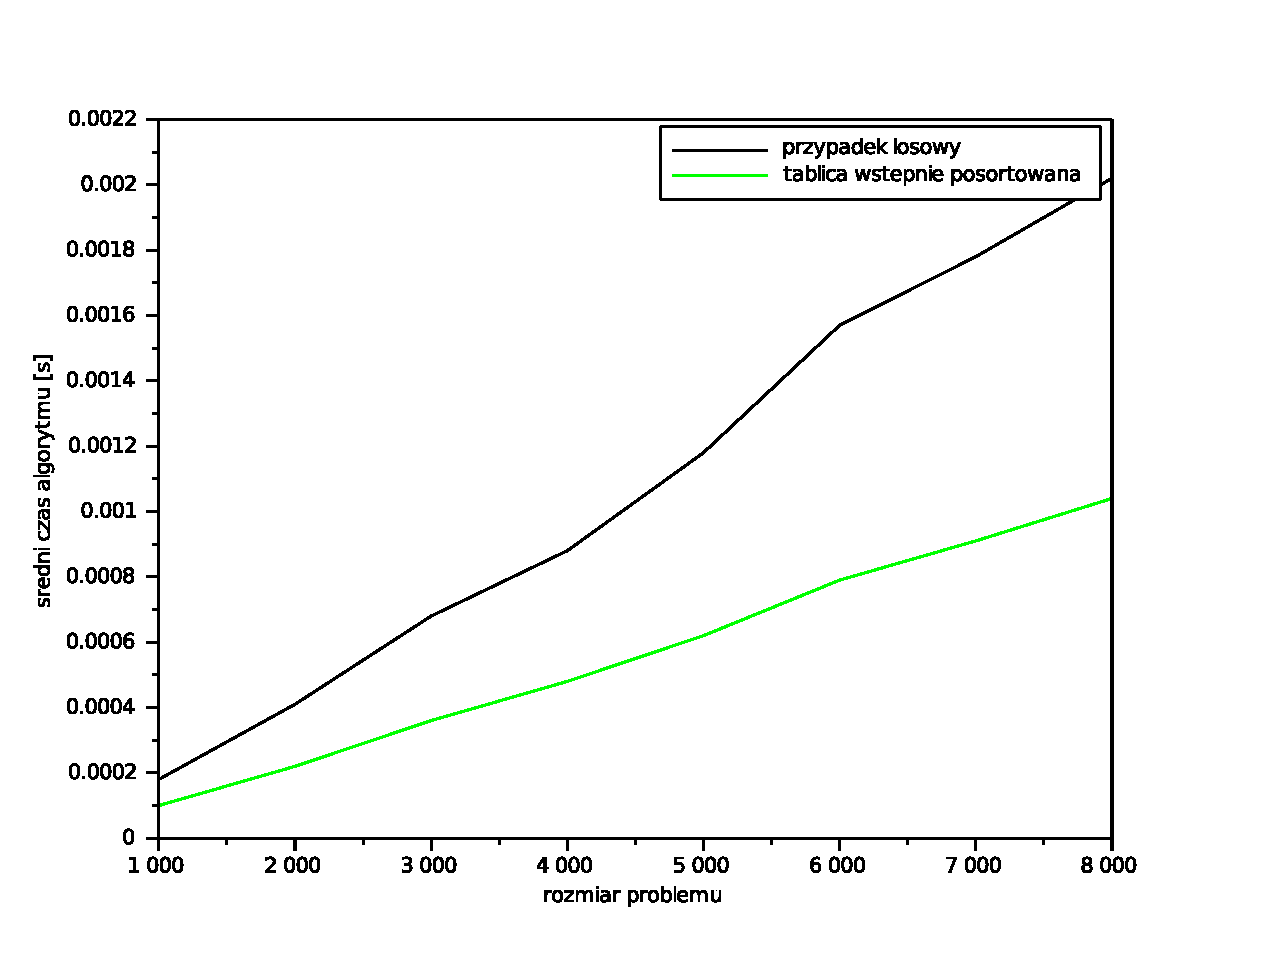
\includegraphics[width=\textwidth]{files/quick.pdf}
\caption{Zależność czasu wykonywania algorytmu od rozmiaru problemu dla sortowania szybkiego. \label{quicksort}} 
\end{figure}


\newpage
\subsection {Sortowanie przez scalanie (mergesort)}
\begin{figure}[!htp]
\centering
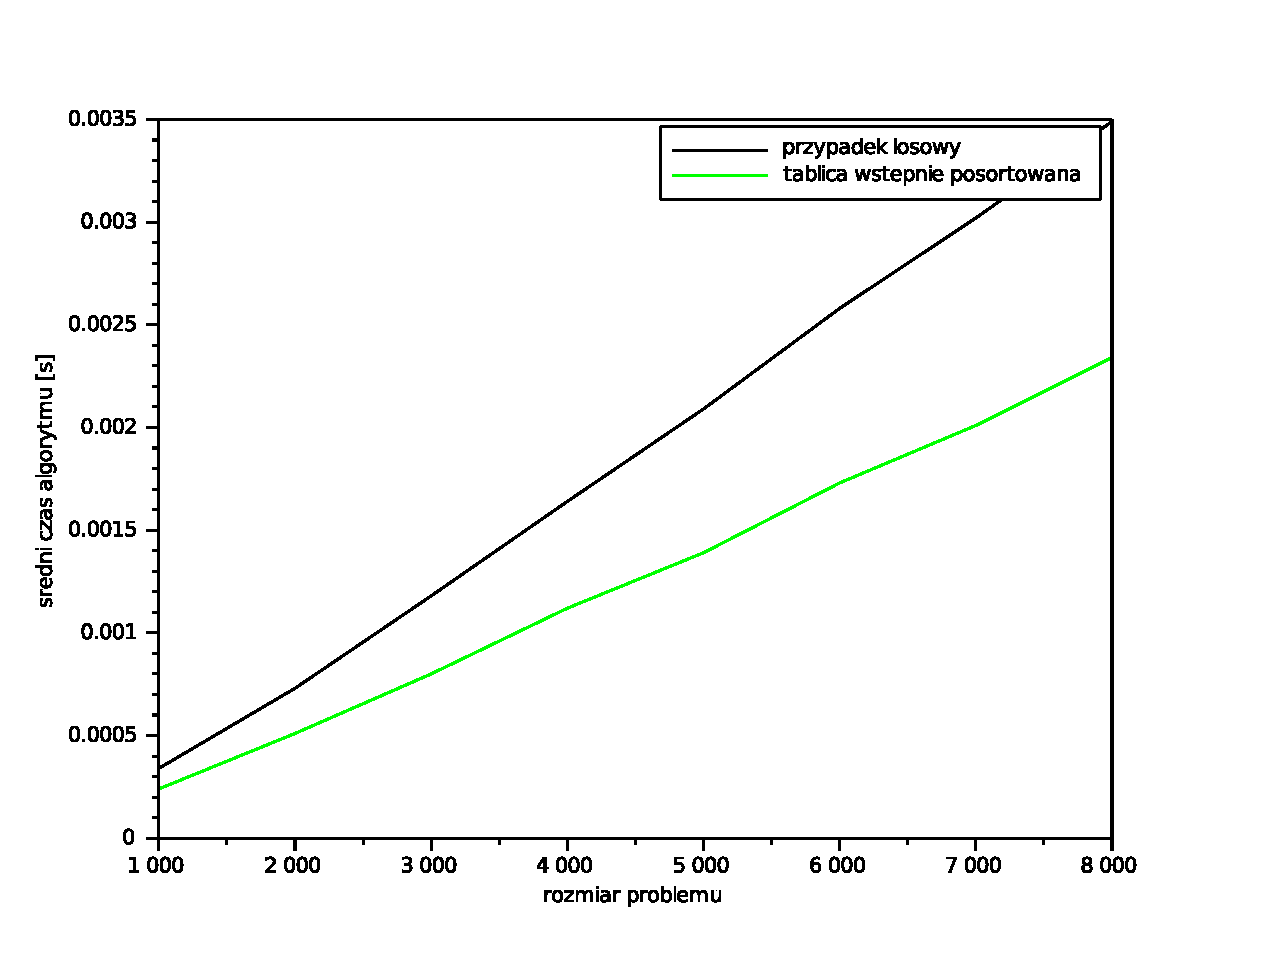
\includegraphics[width=\textwidth]{files/merge.pdf}
\caption{Zależność czasu wykonywania algorytmu od rozmiaru problemu dla sortowania przez scalanie. \label{merge}} 
\end{figure}


\newpage
\subsection {Sortowanie przez kopcowanie (heapsort)}
\begin{figure}[!htp]
\centering
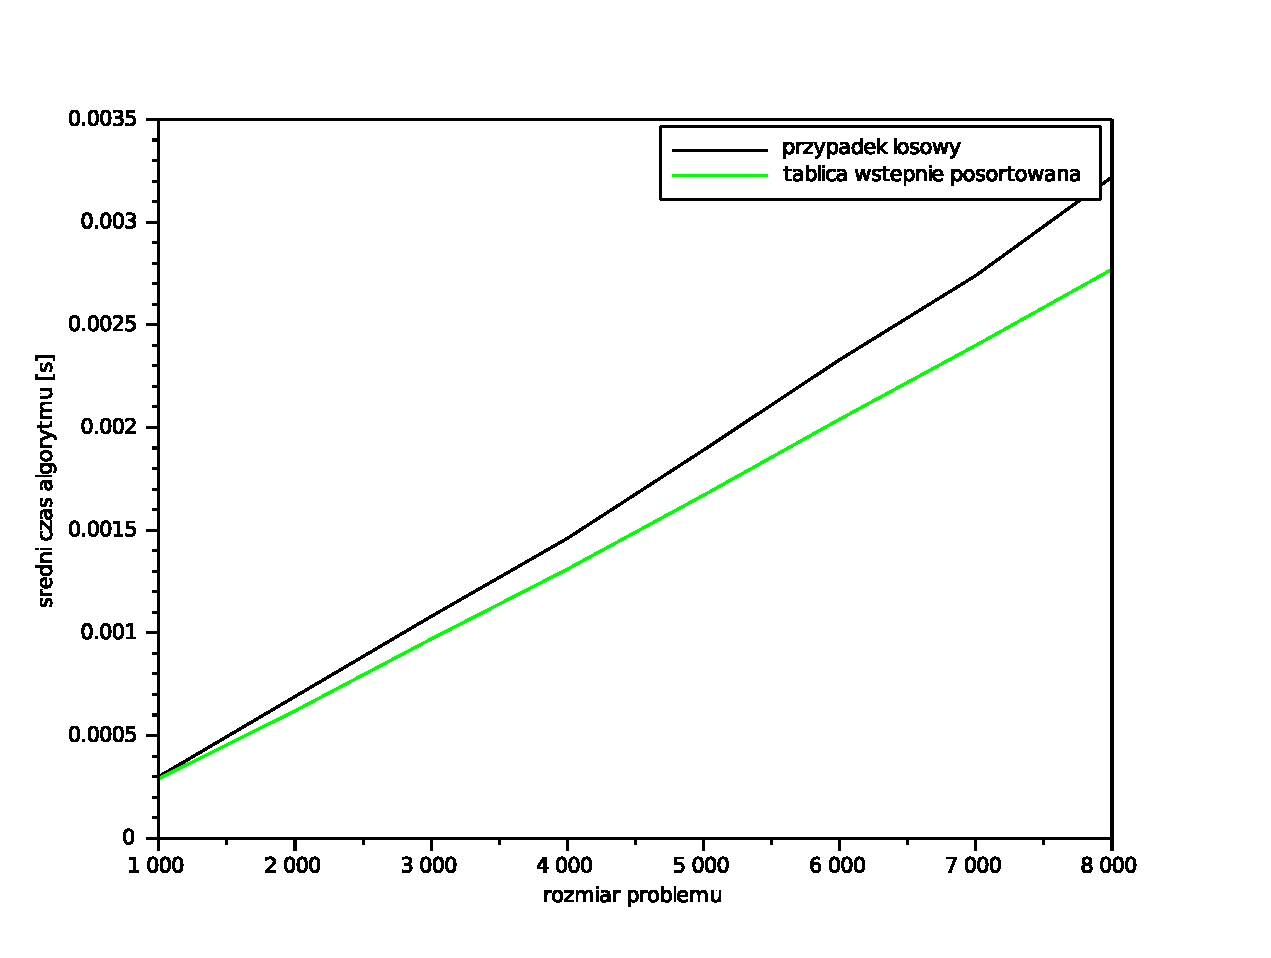
\includegraphics[width=\textwidth]{files/heap.pdf}
\caption{Zależność czasu wykonywania algorytmu od rozmiaru problemu dla sortowania przez kopcowanie. \label{heap}} 
\end{figure}





\newpage
\section{Wnioski\label{wnioski}}
\begin{itemize}
\item Z powyższych wykresów wynika, że wszystkie trzy przetestowane algorytmy są wydajniejsze dla danych wstępnie posortowanych.
\item Średnia czasowa złożoność obliczeniowa dla testowanych algorytmów wynosi O(nlogn)
\end{itemize}

\section{Załączniki}
\begin{itemize}
\item Dokumentacja z Doxygena "Dokumentacja.pdf"
\end{itemize}

\end{document}
